\documentclass{standalone}

\usepackage{xcolor}

\definecolor{myblue}{HTML}{377EB8}
\definecolor{myred}{HTML}{E41A1C}

\usepackage{tikz}
\usepackage{pgfplots}
\pgfplotsset{compat=newest}

\usepackage{lmodern}
\SetSymbolFont{letters}{bold}{OML}{cmbr}{bx}{it}
\renewcommand{\familydefault}{\sfdefault}

\usepackage{sansmathfonts}

\begin{document}
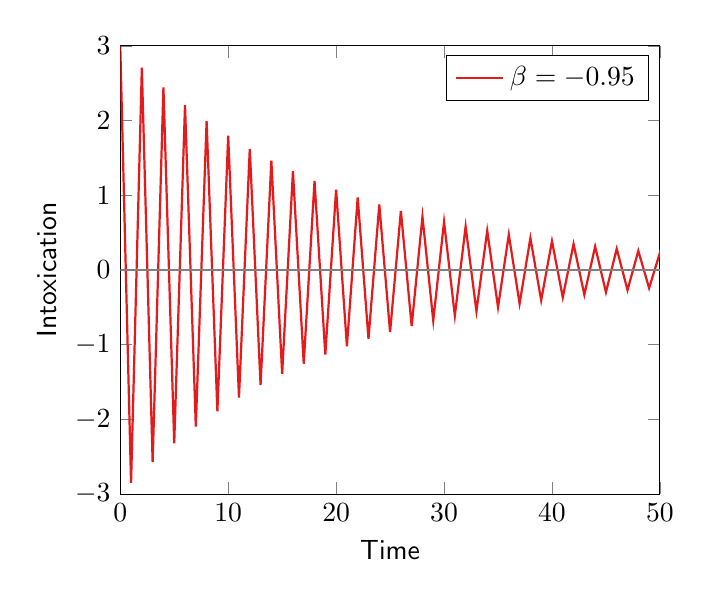
\begin{tikzpicture}
	\begin{axis}[
			xlabel={Time},
			ylabel={Intoxication},
			xmin=0, xmax=50,
			ymin=-3, ymax=3,
			xtick={0,10,20,30,40,50},
			ytick={-3,-2,-1,0,1,2,3},
			grid style=dashed,
		]		
		\addplot[
			color=myred,
            thick
		]
		coordinates {
			(0, 3)
			(1, -2.85)
			(2, 2.7075)
			(3, -2.572125)
			(4, 2.44351875)
			(5, -2.3213428125)
			(6, 2.205275671875)
			(7, -2.09501188828125)
			(8, 1.99026129386719)
			(9, -1.89074822917383)
			(10, 1.79621081771514)
			(11, -1.70640027682938)
			(12, 1.62108026298791)
			(13, -1.54002624983851)
			(14, 1.46302493734659)
			(15, -1.38987369047926)
			(16, 1.3203800059553)
			(17, -1.25436100565753)
			(18, 1.19164295537465)
			(19, -1.13206080760592)
			(20, 1.07545776722563)
			(21, -1.02168487886434)
			(22, 0.970600634921127)
			(23, -0.92207060317507)
			(24, 0.875967073016317)
			(25, -0.832168719365501)
			(26, 0.790560283397226)
			(27, -0.751032269227365)
			(28, 0.713480655765996)
			(29, -0.677806622977696)
			(30, 0.643916291828812)
			(31, -0.611720477237371)
			(32, 0.581134453375502)
			(33, -0.552077730706727)
			(34, 0.524473844171391)
			(35, -0.498250151962821)
			(36, 4.73E-01)
			(37, -4.50E-01)
			(38, 4.27E-01)
			(39, -4.06E-01)
			(40, 3.86E-01)
			(41, -3.66E-01)
			(42, 3.48E-01)
			(43, -3.31E-01)
			(44, 3.14E-01)
			(45, -2.98E-01)
			(46, 2.83E-01)
			(47, -2.69E-01)
			(48, 2.56E-01)
			(49, -2.43E-01)
			(50, 2.31E-01)
			(51, -2.19E-01)
			(52, 2.08E-01)
			(53, -1.98E-01)
			(54, 1.88E-01)
			(55, -1.79E-01)
			(56, 1.70E-01)
			(57, -1.61E-01)
			(58, 1.53E-01)
			(59, -1.45E-01)
			(60, 1.38E-01)
			(61, -1.31E-01)
			(62, 1.25E-01)
			(63, -1.18E-01)
			(64, 1.13E-01)
			(65, -1.07E-01)
			(66, 1.02E-01)
			(67, -9.65E-02)
			(68, 9.17E-02)
			(69, -8.71E-02)
			(70, 8.28E-02)
			(71, -7.86E-02)
			(72, 7.47E-02)
			(73, -7.09E-02)
			(74, 6.74E-02)
			(75, -6.40E-02)
			(76, 6.08E-02)
			(77, -5.78E-02)
			(78, 5.49E-02)
			(79, -5.22E-02)
			(80, 4.95E-02)
			(81, -4.71E-02)
			(82, 4.47E-02)
			(83, -4.25E-02)
			(84, 4.04E-02)
			(85, -3.83E-02)
			(86, 3.64E-02)
			(87, -3.46E-02)
			(88, 3.29E-02)
			(89, -3.12E-02)
			(90, 2.97E-02)
			(91, -2.82E-02)
			(92, 2.68E-02)
			(93, -2.54E-02)
			(94, 2.42E-02)
			(95, -2.30E-02)
			(96, 2.18E-02)
			(97, -2.07E-02)
			(98, 1.97E-02)
			(99, -1.87E-02)
		};
		\draw[gray] (0,0) -- (100,0);
		\legend{$\beta = -0.95$}
	\end{axis}
\end{tikzpicture}
\end{document}

% time <- 100
% beta <- 0.95
% y <- rep(x = NA, times = time)
% y[1] <- +3
% for (i in 2:time) {
%   y[i] <- beta * y[i - 1]
% }
% plot(y, type = "l")
% y
